% !TEX root = ../../thesis.tex

% \cleardoublepage
% \newpage
% \thispagestyle{plain}
% \mbox{}

% \includepdf{/Users/matthieulapeyre/Documents/phd_thesis/media/poppy.pdf}
% \includepdf{/Users/matthieulapeyre/Documents/phd_thesis/media/blueprint}

\chapter{The Poppy development} % (fold)

\section{Motivations} % (fold)

As we highlighted in the chapter\ref{}, using concepts such as morphological computation, passive dynamics and ecological balance seem to be promising for making robot more robust to their environment.
However exploring these concepts require to consider the morphology as an experimental variable and therefore design experimental platform allowing to easily and quickly change it.

We addressed these needs by applying the methodology presented in the chapter\ref{} on the design of a whole new humanoid platform we named Poppy\texttrademark, one of the first 3D printed and open source (software \& hardware)humanoid robot.

The choice of an humanoid platform was motivated by our interest on exploring interaction between the morphology and cognition for biped locomotion.
Also, when we began this work (mid-2012), no other robotic platform was available to easily explore morphological aspect.
Thus we decided to extend the ability of Poppy to the exploration a wider range of scientific challenge such as Human Robot Interaction (HRI), sensorimotor learning, ...
Allowing the Poppy platform to raise its ambition to become a benchmarking platform.

Thanks to our FabLab-inspired approach, the first functional and diffusible prototype has been achieved in just 4 months.
Then a second version occurred to make the robot more versatile and easy to use for non-expert user such as the education and artistic communities.

In this chapter, we will explain the design of Poppy from both a conceptual and a technical point of view.


\section{Design guidelines} % (fold)

\subsubsection{Modular morphology} % (fold)
The whole structure must be easy to reconfigure both for repairing or hacking purpose.
This mean the process to replace a Poppy's part must be simple, low-cost and not require time or special tooling.


\subsubsection{Less is more: keep it simple}

The fact we want to design an easily reproducible robot means we are limited in our design choices.
In most case, finding a simple solution avoid the use of an easy solution: we should minimize the number of part and suppliers, be careful of the availability of our parts in each country, take in account the cost and the assembly complexity.
All these constraints make the design of the robot way more complex than a unique prototype robot.
It also raises some limitation to the main Poppy version while some interesting or efficient solution cannot be kept due to their complexity.


\subsubsection{A lightweight structure and under-actuated} % (fold)

Many humanoid robots use powerful motors often associated with highly accurate sensors.
This has a cost, both in terms of weight and computation resources.
Moreover, to ensure the accuracy of the sensory-motor space it is necessary to design very rigid mechanical parts.
The whole structure obtained is powerful but very heavy and due to inertia not very agile.
This kind of robots can intensively repeat precise and complex movements, but are somewhat uncomfortable when it comes to walking on uneven ground.

All mechanical parts were designed to optimize their weight and make the platform Poppy as light as possible.
The obtained mass reduction allows the use of less powerful motors which are therefore lighter.
We can thus have a lightweight robot, strong and powerful enough to perform tasks such as walking and physical interaction.

Weight reduction was achieved through the use of trellis structures.
These structures, mainly used in civil engineering, are among the best technical solutions to optimize the weight/resistance ratio.
All the limbs of Poppy are based on this structure and have been optimized using finite element analysis (FEA) to perform structural simulation and validate parts performance and safety factors.

\subsubsection{Bio-inspired morphology} % (fold)
Human being is a great example of biped locomotion ability.
Strictly mimicking the human morphology is certainly not a good idea as the element composing a robot are not comparable.
However, studying the functional interest of certain human bio-mechanic properties can reveal interesting insight to explore novel humanoid design.

\subsubsection{Ecological balance principle} % (fold)
The ecological balance principle, introduce by Rolf Pfeifer, states that there is a balance or task distribution between morphology, materials, control, and interaction with the environment.
Following this principle, we try to keep a balance between the different part of the robot.

\subsubsection{Whole body compliance} % (fold)
Important aspects of adaptation to physical obstacles or HRI require humanoid robots to be full-body compliant.
This includes both the ability to absorb external shocks due to the passive compliance of the mechanical structure (bendable materials and springs), but also the ability to actively and dynamically control the compliance of motors, which may be either controlled in position with compliance, or directly in torque (thanks to the use of adequate recent servomotor technologies).

\subsubsection{Take care of the aesthetic} % (fold)
In the scientific community, design and aesthetic are often left aside as a superficial feature.
But when an object has to interact with human, the design and aesthetic are the communication channels.
The interaction with our senses change the way we understand the purpose of a object.

As any communication tool, the message we convey can be noised or enforced by the form.
Thus the robot appearance must fit the robot abilities and try to give insights to the user about what it can or cannot do.

Both at a macro or micro scale, the Poppy aesthetic is thought to show some conceptual aspects of its design.
\begin{itemize}
    \item Modular
    \item Smooth and compliant
    \item Lightweight
    \item Under-actuated
\end{itemize}

We do not hide the stuff, user can see motors, wire...



\section{Poppy overview} % (fold)

Poppy (Fig.~\ref{fig:Poppy_comparaison}) is a 84cm high humanoid robot which weights 3.5kg.
It has a sensorimotor space consisting of 25 motorized joints using Robotis Dynamixel servomotors (MX-28 and AX-12).
These servo-motors give access to a large number of internal sensors and allow tuning dynamically their compliance (see \ref{ssub:robot_actuation}).
The sensors space is extended by the addition of 8 force sensors under each foot, an inertial measurement unit located in the head and two wide-angle HD cameras.
In addition, a 4" LCD screen is located on the face for visual communication (such as emotions, interaction).



In order to develop an adapted mechanical structure, we interested ourselves in how evolution solved sensorimotor task related to locomotion and in particular bipedal locomotion.
As human locomotion represents one of the finest example of mastering bipedal walking, we took functional inspiration of some elements that seem relevant to improve the locomotion of humanoid robots.

\begin{figure}[thpb]
    \centering
    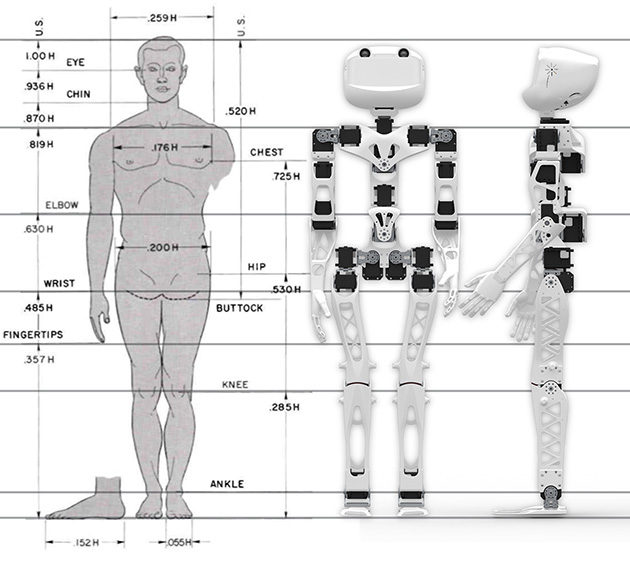
\includegraphics[width=6cm]{proportion_poppy.jpg}
    \caption{Human proportion used for the design of Poppy \cite{dufour2005biomecanique}}
    \label{fig:proportion_poppy}
\end{figure}

This bio-inspiration is expressed on the whole structure of Poppy.
On the anatomical point of view, it reproduces the human proportions as described in the literature \cite{dufour2005biomecanique}  (see Fig.~\ref{fig:proportion_poppy}) and their sensorimotor space organization: i.e.
the main degrees of freedom (actuated and passive), an inertial unit in the head and force sensors distributed underfoot.

As explained in \ref{sec:introduction}, biped locomotion is a central design goal of the Poppy platform.
For this purpose, the morphological optimization is mainly expressed on the locomotive system (legs and trunks) in order to increase the robot robustness, agility and stability during the walking.


\subsection{Lightweight and compliant structure} % (fold)
\label{sub:a_ligthweight_and_compliant_structre}
Many humanoid robots use powerful motors often associated with highly accurate sensors.
This has a cost, both in terms of weight and computation resources.
Moreover, to ensure the accuracy of the sensory-motor space it is necessary to design very rigid mechanical parts.
The whole structure obtained is powerful but very heavy and so not very agile.
This kind of robots can intensively repeat precise and complex movements, but are somewhat uncomfortable when it comes to walking on uneven ground.

Following ecological principles \cite{pfeifer2005new} we decided to design a lightweight and compliant robot requiring low actuation power.
All our design choices, such as the materials, the motors or the sensors, have been made in this direction and to try to tackle the challenges presented in the introduction.
In the next sections we will detail each part of the robot and how they fit within these designs principles.

\subsubsection{Actuation} % (fold)
\label{ssub:robot_actuation}

While emerging technologies such as linear motor, artificial muscle or using both motors and cables are promising, they are still not ``plug'n'play'' solutions (e.g.
require air circuit, associating motor and cable is a complex task, pistons are heavy and slow).
It makes their integration in a small platform such as Poppy difficult.

We therefore chose to use Robotis Dynamixel servo-motors\footnote{\url{http://www.robotis.com/xe/dynamixel_en}} for the robot actuation.
They are all-in-one-modules which contain drivers, encoders and communication lines.
They are also quite powerful, robust and precise.
This is done by the combination of maxon motor, metal gear box and precise position sensor (resolution: 0.1\textsuperscript{o}).
They embed a 32bits micro-controller dedicated to the communication (serial port), the control of the joint (position, speed or torque) and the measurement of severals internal data such as the real position, speed, load or temperature.
They also allow tuning the internal PID or limiting the maximal torque.
This permits rich behaviors useful both for physical interaction and locomotion.
However these motors are quite heavy (72, 126 and 153g respectively for MX-28, MX-64 and MX-106) in comparison of the Futaba servo-motors\footnote{\url{http://www.futaba-rc.com/servos/brushless.html}}, 20-50g for a comparable output torque.
Given these constraints, the challenge consists in minimizing the number of motors and the power needed to reduce the global weight of the robot.

It would be interesting to mix both robotis motors with basic servo-motors where the compliance is not so important.
However, as this makes the design more complex we did not explore this solution yet.

% subsubsection robot_actuation (end)

\subsubsection{Material properties} % (fold)
\label{ssub:material_properties}

All mechanicals parts are made using laser sintering technology.
This 3D printing process allows the production of almost any shape without constraint.
In addition, the price of the part depends on the total size and not on the complexity of the shape.
This permits the production of very optimized shapes without increasing the total price of the robot.
Also, this technique is compatible with several materials from polyamide to titanium.
Parts manufacturing was subcontracted to an external company\footnote{\url{http://i.materialise.com/}}.

For Poppy's structure we decided to use the polyamide material because it is lightweight and very flexible while keeping good strength properties (see the table \ref{tab:materials}).

\begin{table}[h]
    \centering
    \begin{tabularx}{0.8\linewidth }{l X X X}
        Material & Mass Density $\rho$ ($kg/m^3$) &  Yield strength $\sigma$~($MPa$) & Young Modulus $E$($GPa$)\\
        \hline
        Polyamide & $930$ & $49$ & $1.65$\\

        Aluminum & $2700$ & $200$ & $70$\\

        Steel & $7500-8000$ & $350$ & $200$\\

        Titanium & $4500$ & $1200$ & $114$\\

    \end{tabularx}

    \caption{Comparison of material properties.
    The Young modulus represents the stiffness of the material while the yield strength corresponds to the maximal stress tolerable before plastic deformation.}
    \label{tab:materials}
\end{table}


% subsubsection material_properties (end)


\subsubsection{Structure design} % (fold)
\label{ssub:structure_design}


All mechanical parts were designed to optimize their weight and make the platform Poppy as light as possible.
The obtained mass reduction allows the use of less powerful motors which are therefore lighter.
We can thus have a lightweight robot, strong and powerful enough to perform tasks such as walking and physical interaction.

Weight reduction was achieved through the use of trellis structures.
These structures, mainly used in civil engineering, are among the best technical solutions to optimize the weight/resistance ratio.
All the limbs of Poppy are based on this structure and have been optimized using finite element analysis (FEA) to perform structural simulation and validate parts performance and safety factors.

\begin{figure}[thpb]
    \centering
    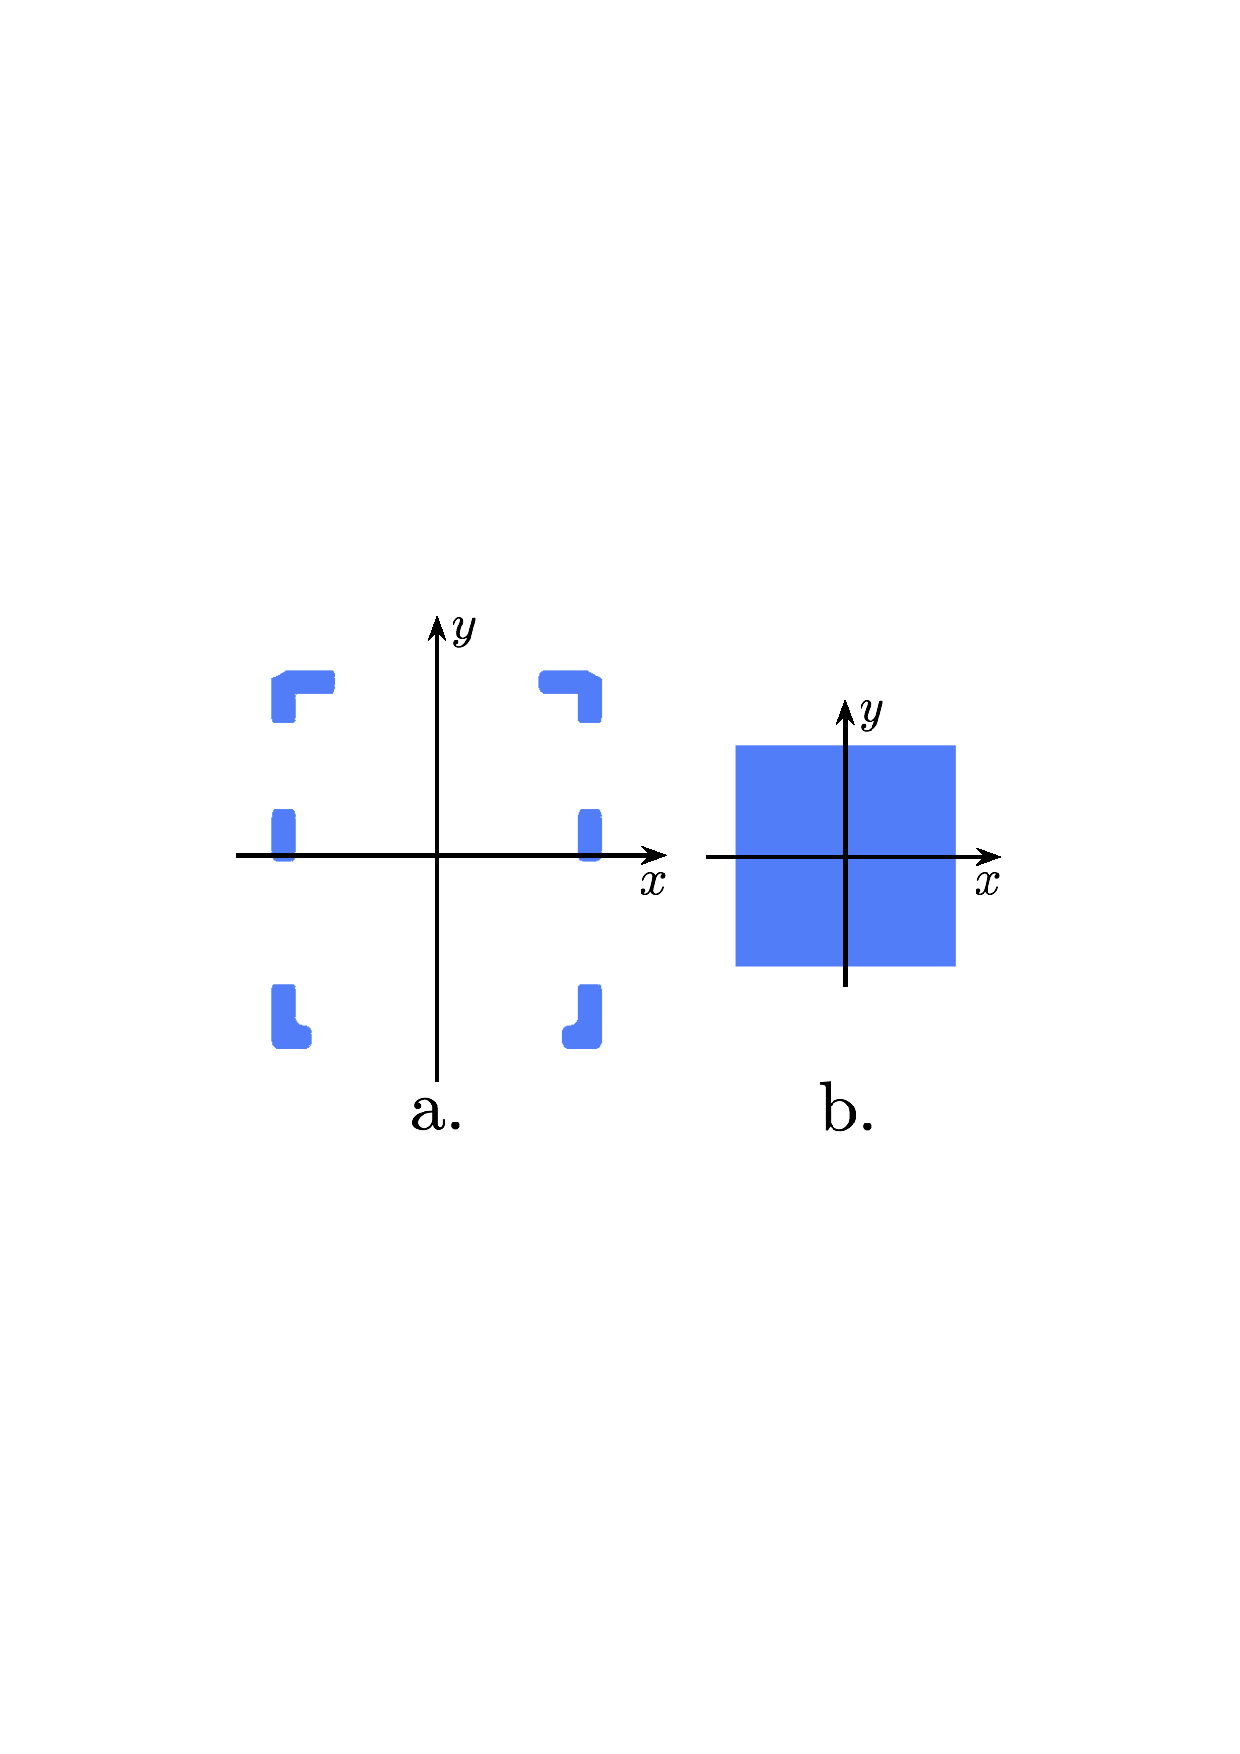
\includegraphics[width=0.5\linewidth]{leg_section.pdf}
    \caption{a.
    Section of the Poppy's leg.
    b.
    Equivalent square section}
    \label{fig:leg_section}
\end{figure}


The main quadratic momentum taken at the middle of the leg given the trellis structure (see Fig.~\ref{fig:leg_section}.a) is:

% \begin{equation}
%     I_x = \iint_s y^2 dxdy
%     % I_y = \iint_s x^2 dxdy
%     % with s = dxdy
% \end{equation}
\begin{center}
    $I_x = 54862 mm^4$
    ,
    $I_y = 53260 mm^4$
\end{center}

For instance, given a solid bar with rectangular profile (Fig.~\ref{fig:leg_section}.b):

{\centering
    $I_x = \frac{b \cdot h^3}{12}$
    ,
    $I_y = \frac{b^3 \cdot h}{12}$

}
It would require a section such as $b=27.72 mm$ and $h=27.59 mm$ to get the same quadratic momentum.
Considering the length of the leg part (i.e.
$190 mm$), the total mass would be equal to $142 g$ instead of $47 g$ for the actual leg.
This corresponds to a reduction of 70\% of the mass.

By using this mesh structure on most of the robot, the total weight of the 3D
printed parts were reduced of about 1.3kg while still being resistant under shocks and falls.


\subsection{The materials} % (fold)
All mechanicals parts are made using laser sintering technology.
This 3D printing process allows the production of almost any shape without constraint.
In addition, the price of the part depends on the total size and not on the complexity of the shape.
This permits the production of very optimized shapes without increasing the total price of the robot.
Also, this technique is compatible with several materials from polyamide to titanium.

For Poppy's structure we decided to use the polyamide material because it is lightweight and very flexible while keeping good strength properties.

\subsection{The actuation} % (fold)

While emerging technologies such as linear motor, artificial muscle or using both motors and cables are promising, they are still not ``plug'n'play'' solutions (e.g.
require air circuit, associating motor and cable is a complex task, pistons are heavy and slow).
It makes their integration in a small platform such as Poppy difficult.

We therefore chose to use Robotis Dynamixel servo-motors\footnote{\url{http://www.robotis.com/xe/dynamixel_en}} for the robot actuation.


\subsection{Electronics} % (fold)
Arduino based.
Off the shelf sensors.






\section{Designed to explore the biped locomotion}

\subsection{Foot design} % (fold)
To allow efficient and human-like walking gait, Poppy's feet design takes some functional inspiration from the actual human foot such as the proportion, compliance and toes which are key features concerning both the human walking and biped robots with a human-like gait.
In addition, we wanted to reduce the weight (i.e.
reducing inertia) of the feet to increase the robot agility.

To keep the foot as light as possible while conserving functional properties we decided to use a single motor for the main motion (sagittal plane) while other DoF are passives.

\subsection{A composite semi-passive ankle} % (fold)
The lateral motion of the foot is limited: few range of motion, low torque.
The need of a 360 deg and high torque motor seems over rated.
Technically the addition of a motor lead to a major weight gain.
We preferred to design  instead a passive joint based on a composite material assembly allowing both robustness and lightness.


\subsection{The hip} % (fold)
Poppy's small feet increase the challenge of the balance of the robot.
Also, to keep the projection of the center of gravity (CoG) inside the support polygon, defined by the feet geometry, it is necessary to control the weight distribution of the robot structure.
In particular, we wanted that in its initial upright posture, Poppy stays balanced without any control.
 Robotis actuators are among the densest elements in the Poppy platform ($ 1700 kg.m^{3} $) and are the main source of weight ($1.8 kg$).
 Their spatial distribution represents therefore the major part of the distribution of masses in Poppy.
In order to limit the displacement of the mass on the back of the robot, we decided to avoid conventional ball joint assembly for the hip joint such that it is made on most robots based on Robotis motors (i.e.
distributed in a plane parallel to the sagittal plane).
Instead, we placed them on the frontal plane as the from left to right stability is greater than the from rear to front stability.
By doing so, the hip joint is not a real ball joint anymore.
Yet, the lost freedom is not relevant for the walking gait.

\subsection{The bio-inspired thigh} % (fold)
If we look closely at the human morphology of the femur, it appears that it is inclined of 6 degrees.
This makes the feet closer to the projection of the center of gravity (see Fig.~\ref{fig:human_thigh}.a).
We reproduced this on Poppy.


\subsection{The knee locking} % (fold)
The Poppy platform involves a semi-passive knee based on the use of additional springs in parallel of the joint actuation.
These springs have been design to participate in the leg dynamic during two main phases:
\begin{itemize}
    \item They help to keep the leg straight during the support phase without any motor control.
    \item During the swing phase, they participate to the flexion of the leg.
\end{itemize}

\subsection{A multi-articulated trunk} % (fold)
Poppy uses the bio-inspired trunk system introduced by Acroban.
Using five servo-motors, it allows the reproduction of the main DOFs of the human spine.
This feature permits the integration of more natural and fluid motion while improving the user experience during physical interaction.
In addition, the spine plays a fundamental role in bipedal walking and postural balance by actively participating in the balancing of the robot.

Contrary to the design of the hips, it was not possible here to fit the 5 motors in the frontal plane due to the limited space in the trunk.
So to reduce the shifting of the center of gravity to the back of the robot we gradually shifted the upper body to the front.
By doing so, we keep the CoG in the support polygon.



\section{Physical and Social interaction} % (fold)



\subsection{The head} % (fold)

\subsection{Underpowered and compliant for safety} % (fold)



\section{Electronic architecture} % (fold)




\section{A versatile control library: pypot} % (fold)
Right from the beginning of the poppy platform development with started the development of a new python library to control the robot.

Following the hardware guidelines, the pypot library was developed to be robust, versatile and easy to use.


\subsection{Why not using ROS ?} % (fold)
One of our main preoccupation is to develop an easy to use research tools.
In this context, we designed pypot to be multi OS compatible.
ROS is a great software but until now, it is really difficult to set up and need a specific Ubuntu version.
Also this software is very greedy which would make its integration difficult in a small robot.

We prefer an interface with ROS.

\subsection{The primitive architecture: The Good, the Bad and the Ugly} % (fold)
The high level design allows the use of primitives.
Primitives are ...

This features is really powerful has it allows to create complex behavior as a sum of simple behavior.


However the interaction between them is tricky and can lead to undesired behavior.



\section{Conclusions} % (fold)

Thanks to the methodology presented in the previous chapter, we were able to develop a first functional version of Poppy in only 4 months.

\section{Limitations} % (fold)



